
%Quille pendulaire
La conception des voiliers de course, dans un contexte de forte compétitivité sportive et technique, utilise toutes les évolutions récentes afin d’améliorer performances et sécurité. Dès les premiers stades de la conception du navire, l’architecte naval intègre les exigences des différents spécialistes qui collaborent au projet. À ce titre la conception d’un voilier de course océanique est analogue à la conduite d’un projet industriel classique où les intervenants s’inscrivent dans une démarche collaborative pilotée par un coordonnateur du projet.

L’étude proposée s’intéresse à quelques aspects de la conception d’une quille pendulaire équipant un monocoque 60’ IMOCA.

%1
\section{Analyse fonctionnelle et structurelle}

%1.1
\subsection{Fonction de la quille dans la dynamique d’un voilier}
Le comportement dynamique d’un voilier est conditionné par ses interactions avec les deux fluides avec lesquels il entre en contact : l’air et l’eau. Il reçoit de l’énergie sous la forme des actions aérodynamiques dues au mouvement relatif air/voiles. Ces actions mécaniques le font avancer et provoquent son inclinaison autour de son axe longitudinal (axe de direction  $\vect{z_N}$ sur la figure \ref{fig_01_quille}). C’est le phénomène de gîte. Pour contrebalancer ce mouvement et éviter que le voilier ne se couche sur l’eau, la quille joue le rôle de contrepoids. Cette quille est généralement constituée d’un voile immergé dans l’eau à l’extrémité duquel se trouve un lest profilé. L’efficacité de la quille dépend de la masse du lest et de la longueur du voile. Ces deux paramètres présentent des limitations : le lest ne peut être trop important sous peine de solliciter dangereusement le voile de quille et la longueur de quille est limitée par le tirant d’eau maximal admissible (il faut permettre l’entrée dans les ports sans toucher le fond !).


\begin{minipage}[b]{.47\linewidth}
%\begin{figure}[!h]
%\centering
\begin{center}
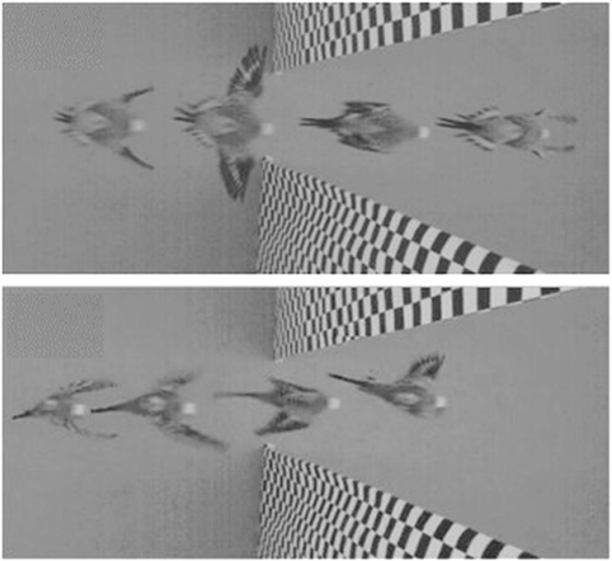
\includegraphics[width=.95\linewidth]{fig_01}
\captionof{figure}{Voilier 60’ IMOCA -- Image Cabinet Finot-Conq \label{fig_01_quille}}
\end{center}
\end{minipage} \hfill
\begin{minipage}[b]{.47\linewidth}
\begin{center}
%\centering
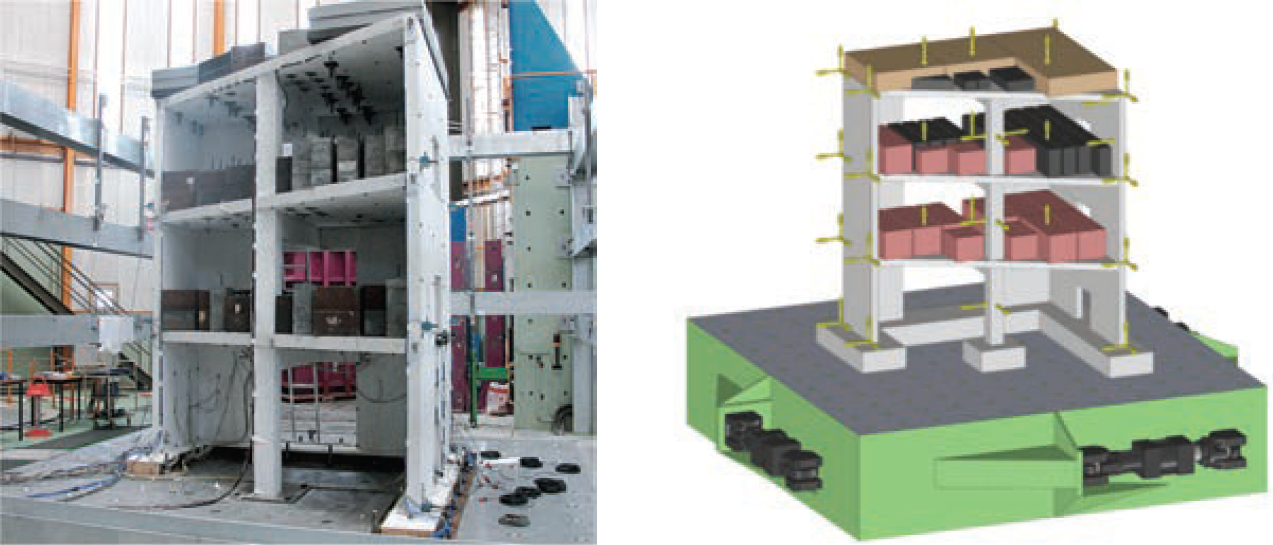
\includegraphics[width=.95\linewidth]{fig_03}
\captionof{figure}{Modèle numérique d’une coque de 60’ IMOCA \label{fig_03_quille}}
\end{center}
 \end{minipage}
 
%1.2 
\subsection{Etude de la stabilité « de formes » d’un voilier doté d’une quille non pendulaire (voir figures 2a et 2b).}

On considère le navire à l’arrêt et en équilibre sur un plan d’eau au repos (figure \ref{fig_02_quille} gauche ). Il est soumis :
\begin{itemize}
\item aux effets de pesanteur représentés par le torseur $\torseurl{-Mg\vect{y}}{\vect{0}}{G}$. $G$ désigne le centre de gravité du navire, $M$ sa masse, $g$ l’accélération de pesanteur et $\vect{y}$ oriente la verticale ascendante du lieu; 
\item aux actions de l’eau sur la coque ou « Poussée d’Archimède » représentées par le torseur : $\torseurl{R_D\vect{y}}{\vect{0}}{C}$. $C$ désigne le centre de carène et $R_D$, exprimée en $N$,  l’intensité  de la résultante des actions de l’eau sur la coque, qu’en construction navale on nomme « déplacement ». À l’équilibre : $R_D = Mg$.
\end{itemize}

\begin{minipage}[c]{.47\linewidth}
%\begin{figure}[H]
%\centering
\begin{center}
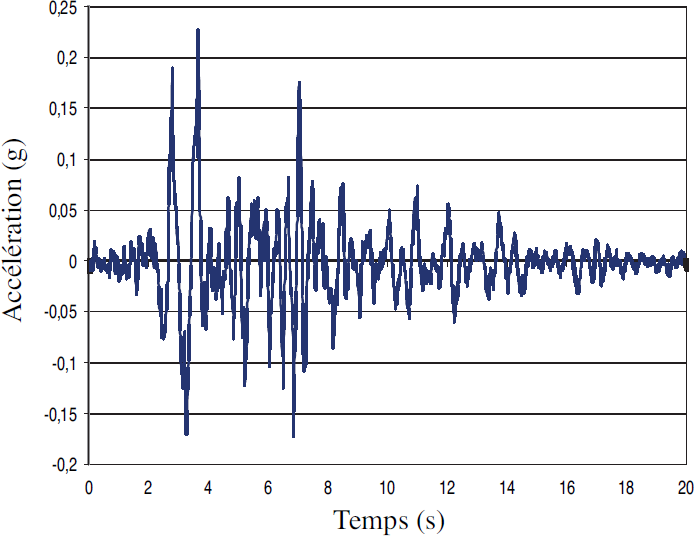
\includegraphics[width=.95\linewidth]{fig_02}
\captionof{figure}{Stabilité << de formes >> \label{fig_02_quille}}
\end{center}
\end{minipage} \hfill
\begin{minipage}[c]{.47\linewidth}
\begin{center}
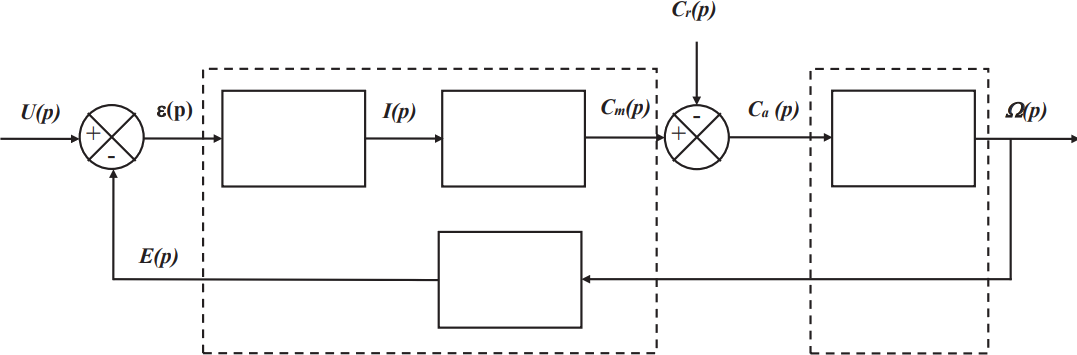
\includegraphics[width=.95\linewidth]{dr_01}
%\caption{Stabilité << de formes >> \label{fig_02_quille}}
\end{center}
\end{minipage}
Une cause extérieure représentée par le torseur $\torseurstat{T}{\text{ext}}{\text{nav}}$, comme l’effet du vent sur les voiles ou des vagues sur la coque, provoque la gîte du navire caractérisée par l’angle de gîte $\alpha=\angl{{y_N}}{{y}}$  (figure \ref{fig_02_quille} droite).

Un nouvel équilibre est alors obtenu sous l’effet des deux actions mécaniques précédentes, le poids et la poussée d’Archimède, ainsi que l’action mécanique extérieure cause de gîte.
L’équation de moment en $G$ selon $\vect{z}$ se traduit par : $\vectm{G}{\text{ext}}{\text{nav}}\cdot \vect{z} + R_D G_x = 0$.

$G_x$ désigne la longueur mesurée algébriquement selon $\vect{x}$ entre le centre de gravité et le centre de carène.
La quantité $R_D G_x$ est appelée :
\begin{itemize}
\item « Moment de redressement » si $R_D G_x > 0$ et $\alpha > 0$ ou $R_D G_x < 0$ et $\alpha < 0$;
\item « Moment de chavirage»        si $R_D G_x< 0$ et $\alpha > 0$ ou $R_D G_x > 0$ et $\alpha < 0$.
\end{itemize}
Dans son avant-projet, l’architecte naval étudie cette stabilité du navire à l’aide d’outils de simulation numérique. À partir du modèle numérique des formes de la coque (exemple figure \ref{fig_03_quille}) et d’une répartition des masses aussi proche que possible de la répartition finale, les différentes positions d’équilibre du navire sont recherchées en fonction de l’angle de gîte. Cette étude fournit une courbe de stabilité théorique où apparaît en abscisse l’angle de gîte $\alpha$ et en ordonnée le paramètre $G_x$ (voir courbe de la figure R1 ci-dessus ou la figure \ref{fig_05_quille}).





%Question 1
La figure R1 donne la courbe de stabilité théorique d’un voilier à quille non pendulaire (quille fixe par rapport à la coque). 

\question{}
\vspace{-.4cm}
\textit{
\begin{enumerate}
\item Expliquer pourquoi $G_x$ suffit à caractériser le moment de redressement ou de chavirage.
\item Pour chaque point d’équilibre repéré sur la courbe par A, B, C, D, E et F, donner dans la case prévue sur la copie le numéro de la figure représentant la position d’équilibre correspondant.
\end{enumerate}}

\begin{center}
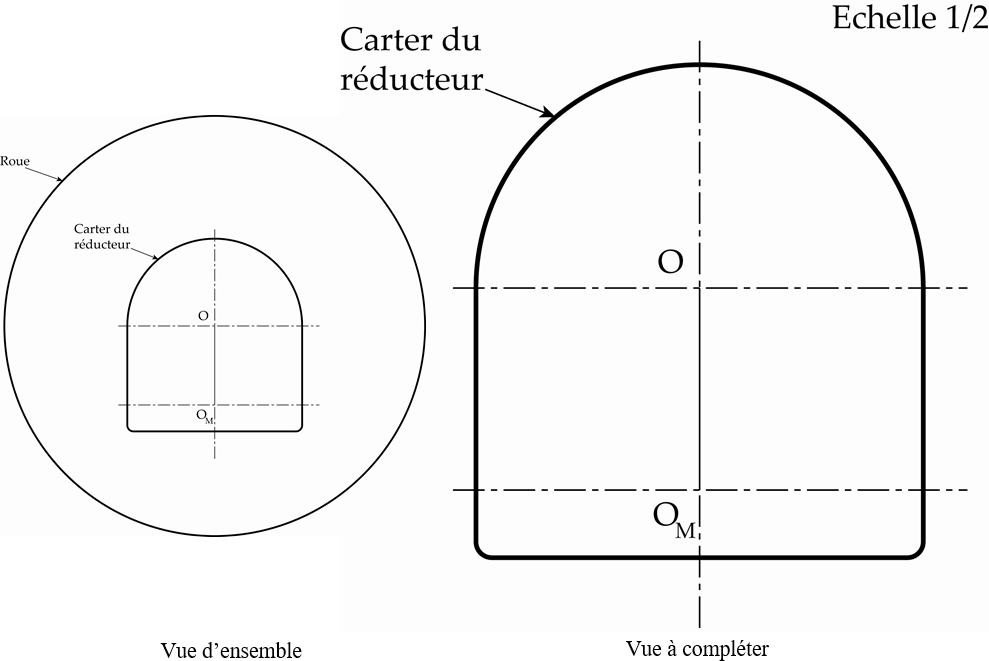
\includegraphics[width=.95\linewidth]{dr_02}
%\caption{Stabilité << de formes >> \label{fig_02_quille}}
\end{center}

\vspace{.5cm}

%Question 2
 En utilisant la modélisation de la figure \ref{fig_04_quille} où on admettra (hypothèse simplificatrice) que le mouvement du navire par rapport au repère galiléen $\repere{H}{x}{y}{z}$ est une rotation d’axe $\axe{H}{z}$, $H$ tel que $\vect{GH}=K\vect{y_N}$ et $L$ constante positive), répondre aux questions suivantes. 

\vspace{.5cm}

\question{}
\vspace{-.4cm}
\textit{
\begin{enumerate}
\item Exprimer la puissance galiléenne des actions de pesanteur développées par le mouvement du navire (rotation d’axe $\axe{H}{z}$) en fonction de $\alpha$, $\dfrac{\d \alpha}{\d t}$, $g$, $M$ et autres paramètres géométriques utiles.
\item Montrer alors que le travail de ces actions de pesanteur est proportionnel à $S_{ij}$
 tel que $S_{ij}=\int\limits_{\alpha_i}^{\alpha_j} Gx (\alpha)\d \alpha$, lorsque l’angle de gîte passe de la valeur $\alpha_i$ à la valeur $\alpha_j$.
\end{enumerate}}

\vspace{.5cm}

\begin{minipage}[b]{.47\linewidth}
\begin{center}
%\centering
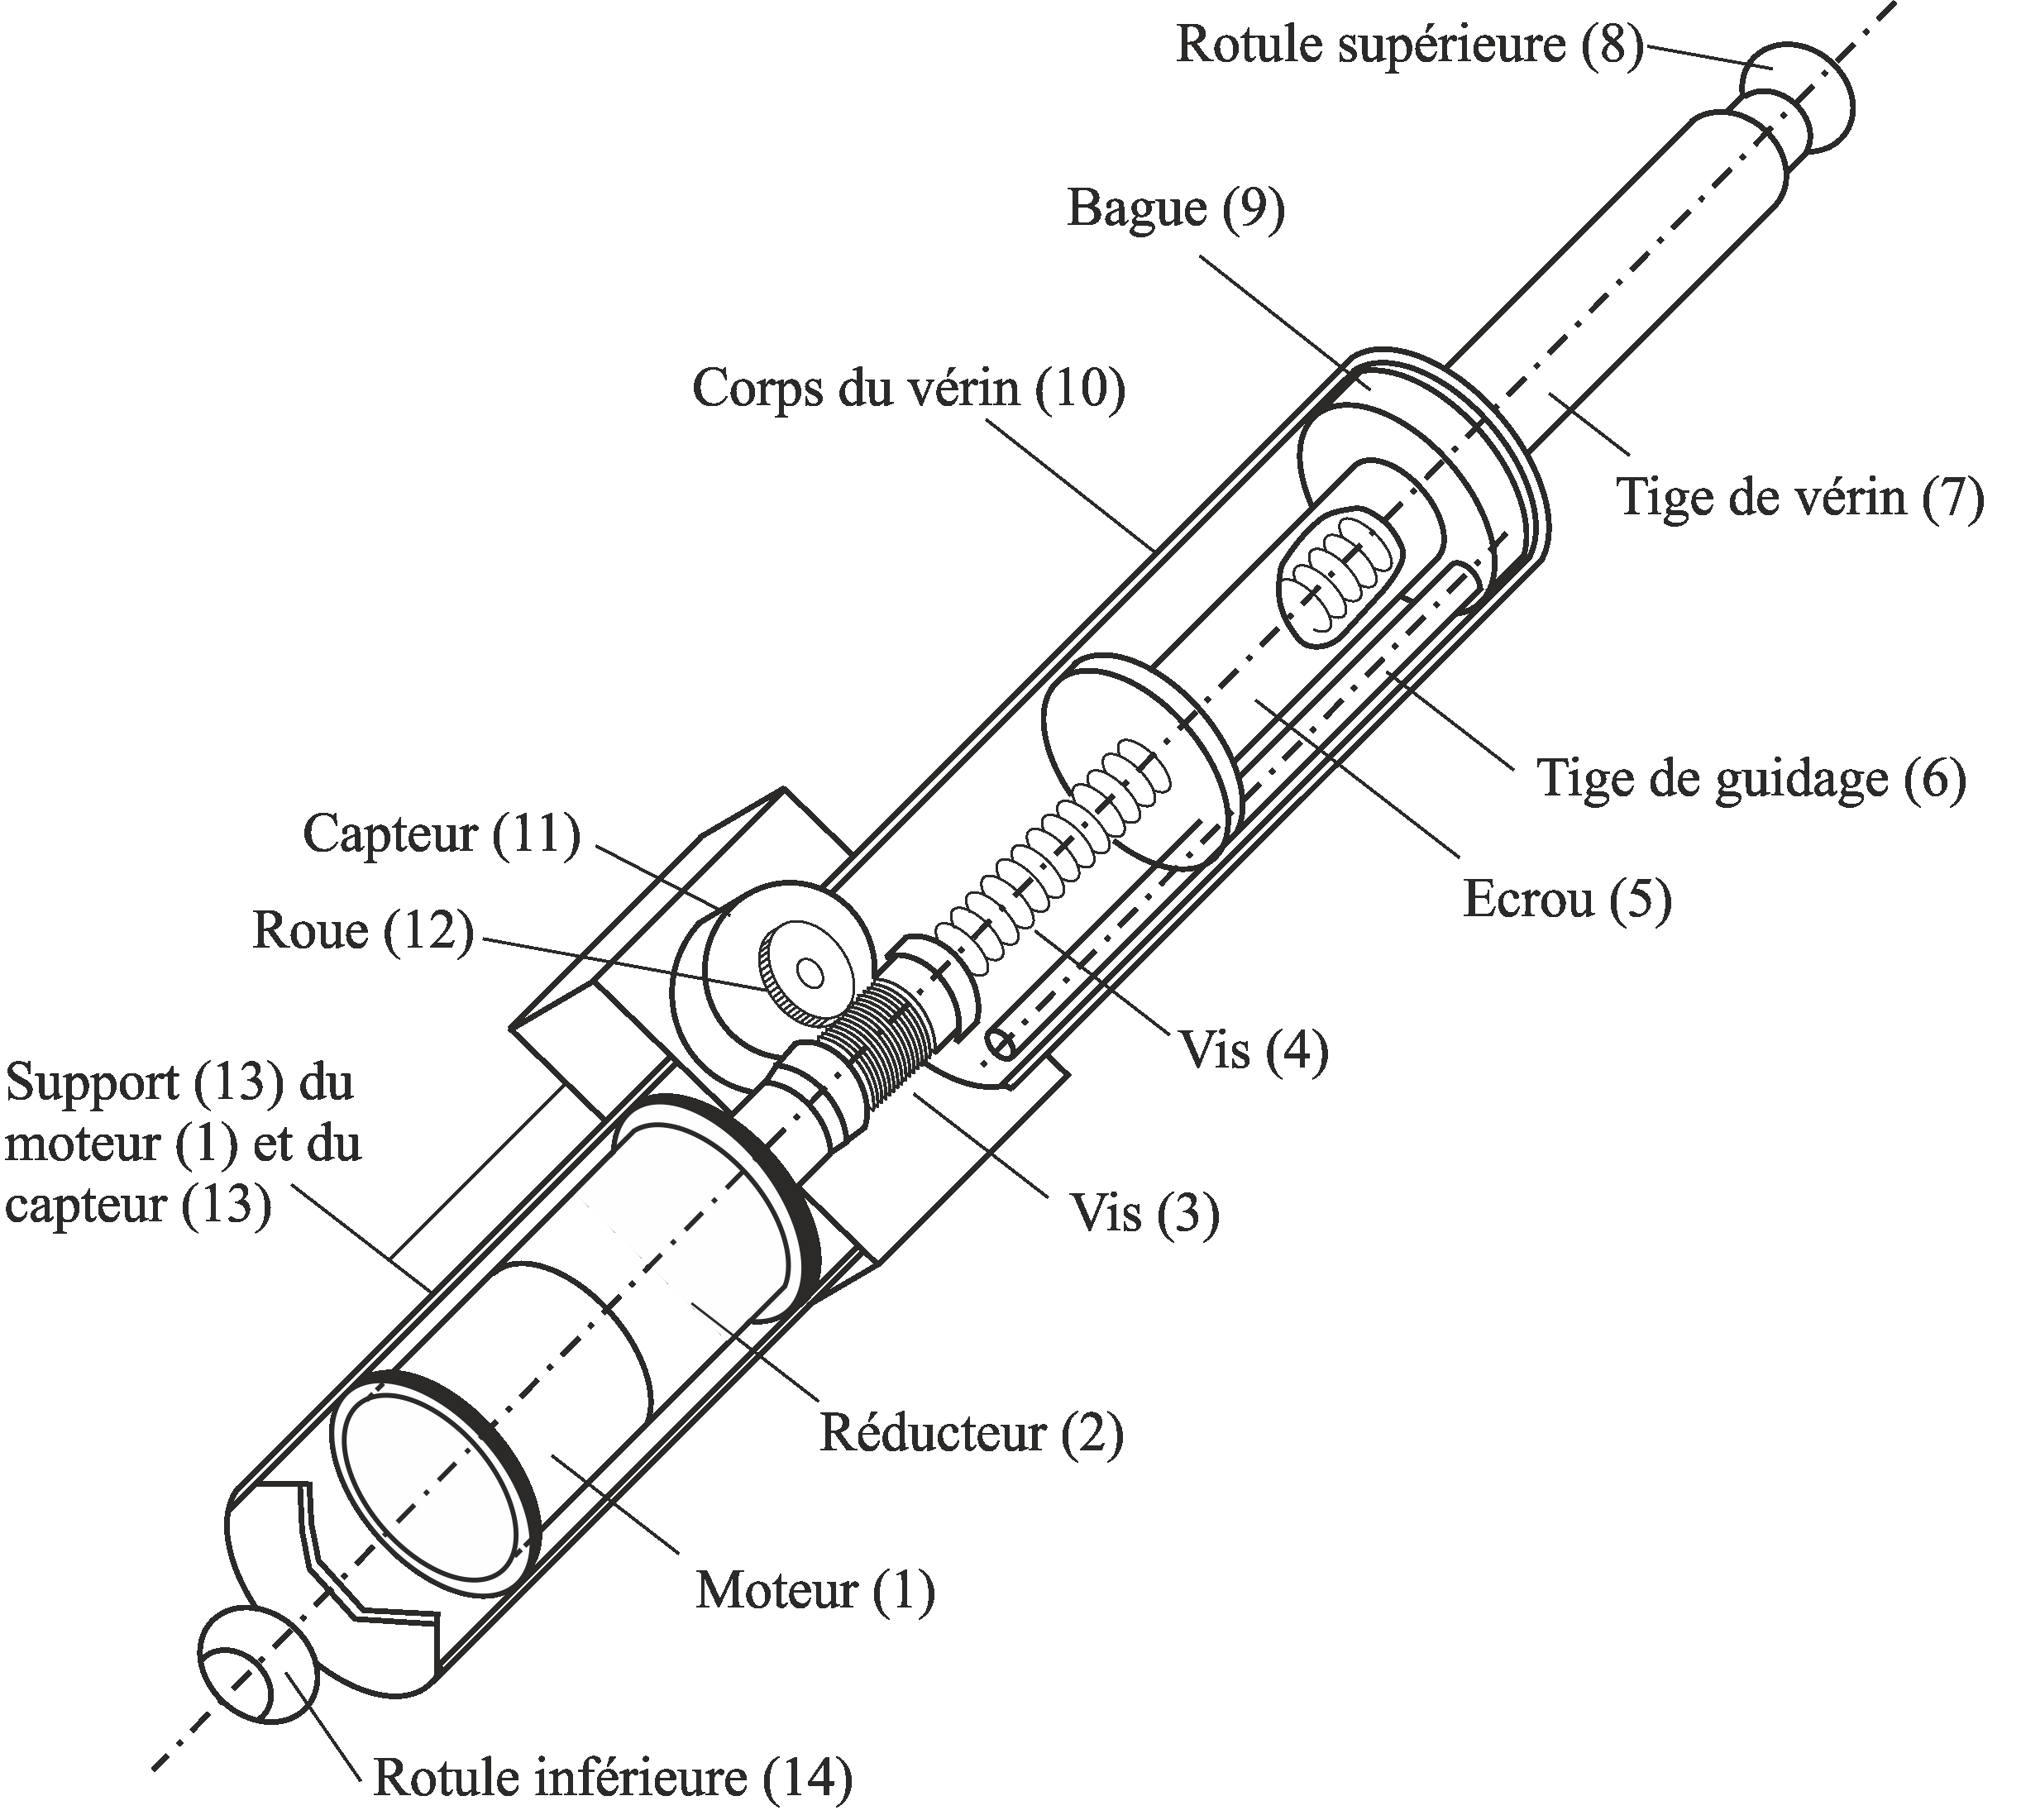
\includegraphics[width=.7\linewidth]{fig_04}
\captionof{figure}{Modélisation du voilier à la gîte \label{fig_04_quille}}
\end{center}
\end{minipage}\hfill
\begin{minipage}[b]{.47\linewidth}
\begin{center}
%\centering
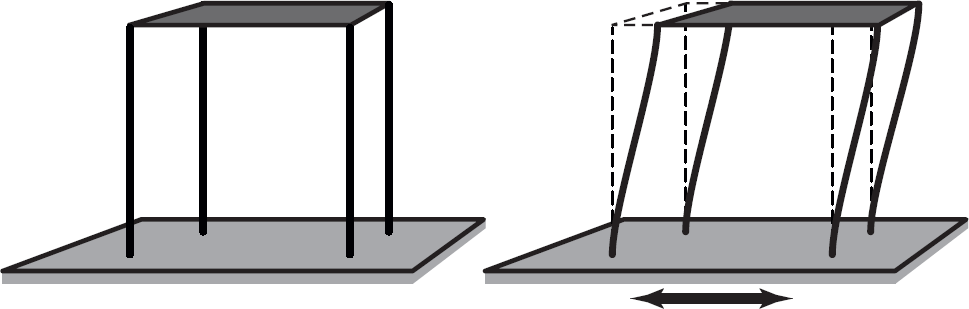
\includegraphics[width=.95\linewidth]{fig_05}
\captionof{figure}{Courbe de stabilité théorique : définition des « aires » $S_{01}$ et $S_{12}$ \label{fig_05_quille}}
\end{center}
 \end{minipage}
 

La figure \ref{fig_05_quille} représente l’évolution, pour un navire 60’ IMOCA à quille fixe, de Gx en fonction de l’angle de gîte $\alpha$, pour $\alpha$ variant de 0 à 180\degres. Sur cette courbe, les quantités 
$S_{01}=\int\limits_{0}^{\alpha_1} Gx(\alpha) \d \alpha$ et 
$S_{12}=\int\limits_{\alpha_1}^{\alpha_2} Gx(\alpha) \d \alpha$  
 sont représentées par les « aires » comprises entre la courbe et l’axe des abscisses.
 
La réglementation impose à l’architecte naval de créer des formes de coque pour lesquelles :
\begin{itemize}
\item l’angle de gîte provoquant la mise en situation de chavirage du voilier (changement de signe de $Gx$) soit au minimum de 120\degres;
\item le rapport des « aires » soit tel que : $\dfrac{S_{01}}{S_{12}}=\dfrac{5}{1}$.
\end{itemize}

%Question 3 
\question{Quel est le sens donné à chacune de ces deux clauses du cahier des charges imposées par le législateur ?}



%1.3 
\subsection{Intérêt d’une quille pendulaire}

Une évolution récente des voiliers de course océanique a été de les doter d’une quille pendulaire (figures \ref{fig_06_quille} et \ref{fig_07_quille}). Cette quille est en liaison pivot d’axe $\axe{O}{z_N}$ avec la coque du navire et peut être orientée d’un côté ou de l’autre du navire. Une fois l’orientation désirée obtenue, tout mouvement dans la liaison pivot est supprimé par le blocage en rotation de celle-ci. La mise en mouvement et le blocage en position de la quille sont réalisés par des chaînes d’énergie et d’information étudiées dans la suite du sujet. 

\begin{minipage}[b]{.47\linewidth}
\begin{center}
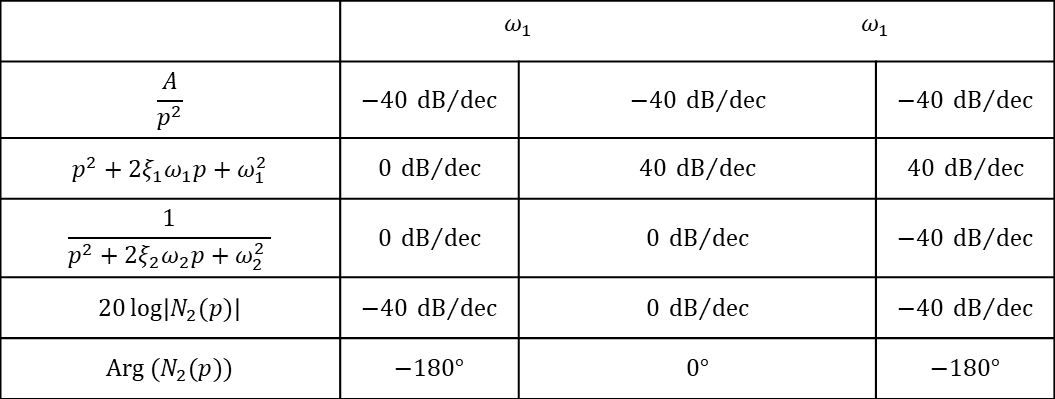
\includegraphics[width=.95\linewidth]{fig_06}
\captionof{figure}{Voilier avec sa quille pendulaire écartée au maximum sur « bâbord » \label{fig_06_quille}}
\end{center}
\end{minipage}\hfill
\begin{minipage}[b]{.47\linewidth}
\begin{center}
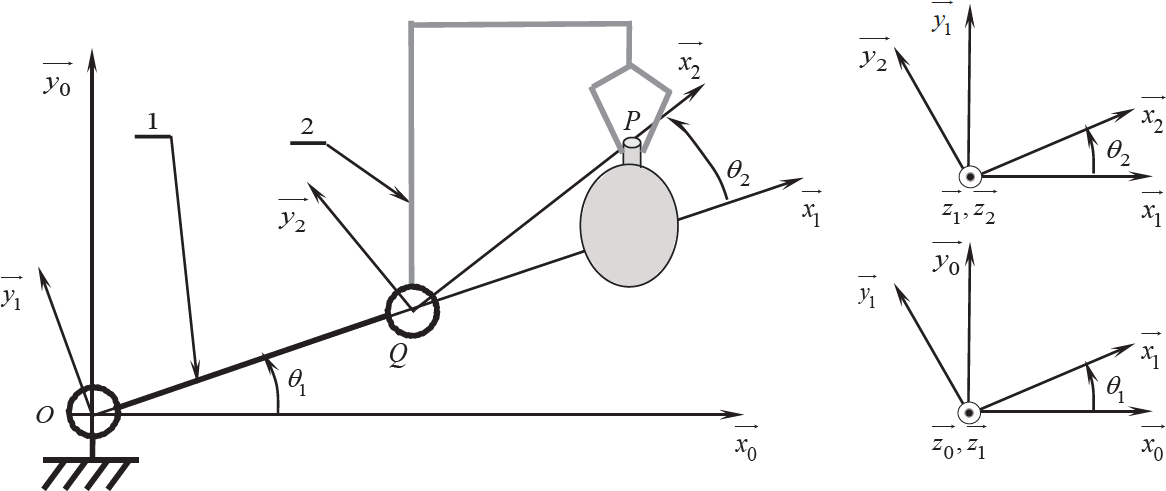
\includegraphics[width=.95\linewidth]{fig_07}
\captionof{figure}{Modèle cinématique élémentaire de la quille pendulaire \label{fig_07_quille}}
\end{center}
 \end{minipage}


La figure R3  donne les courbes de stabilité théorique d’un voilier dont la quille pendulaire est inclinée :
\begin{itemize}
\item au maximum sur « tribord» (à droite dans le sens de la marche) (courbe 1). 
\item d’un angle nul (courbe 2).
\end{itemize}

\begin{center}
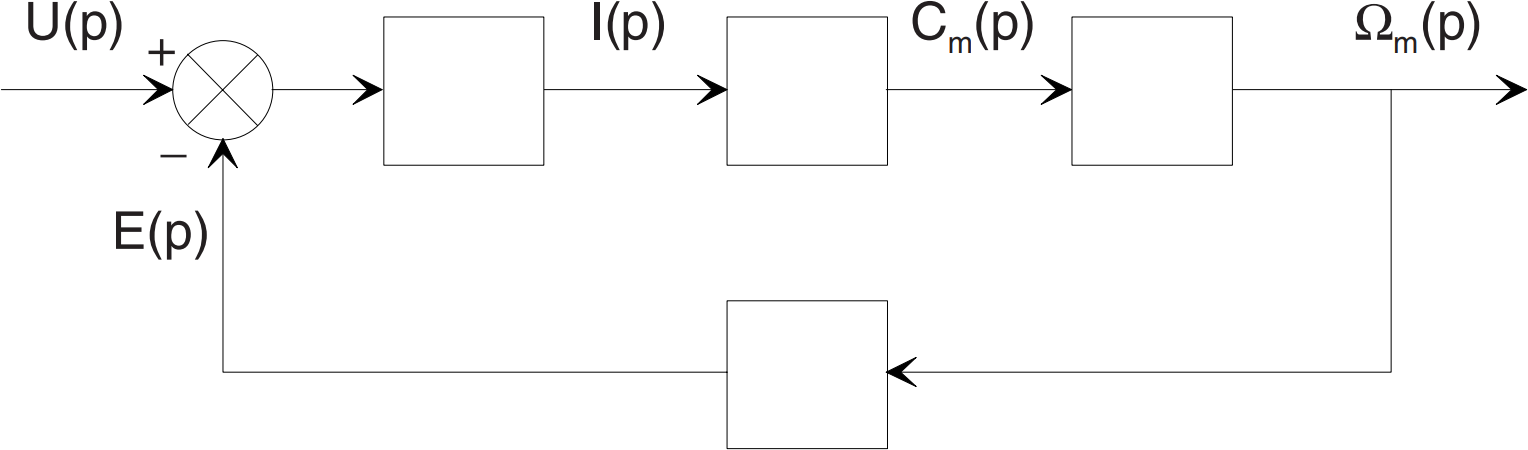
\includegraphics[width=.95\linewidth]{dr_03}
%\caption{Stabilité << de formes >> \label{fig_02_quille}}
\end{center}

\vspace{.5cm}

%Question 4 : 
\question{}
\vspace{-.4cm}
\textit{
\begin{enumerate}
\item Au vu de ces courbes, quels avantages procure la quille pendulaire au comportement du navire lorsqu’il gîte avec un angle $\alpha$ positif ?
\item Pour un angle de gîte $\alpha$ négatif, quel est l’apport de la quille pendulaire ?
\item Dans la situation de navigation où le vent vient de tribord et où la gîte ne doit pas être trop importante malgré la grande surface de voile déployée, quelle doit être la configuration de navigation à adopter ?
\item Répondre par un dessin reproduisant la figure \ref{fig_07_quille} et justifier votre choix. 
\item Lorsque le navire (quille à tribord) est dans la position inappropriée où $\alpha = 180\degres$
indiquer son comportement si une cause extérieure tend à l’écarter de cette position pour l’amener à une
position définie par $\alpha *$ (envisager les deux possibilités : $\alpha *<180\degres$ et 
$\alpha *>180\degres$).
\end{enumerate}}

\vspace{.5cm}

La quille pendulaire constitue un système dont la fonction principale est FP1 : « Orienter la quille ». La composition de cette fonction peut être illustrée par le diagramme F.A.S.T. représenté ci-dessous figure \ref{fig_08_quille}.
 
\begin{center}
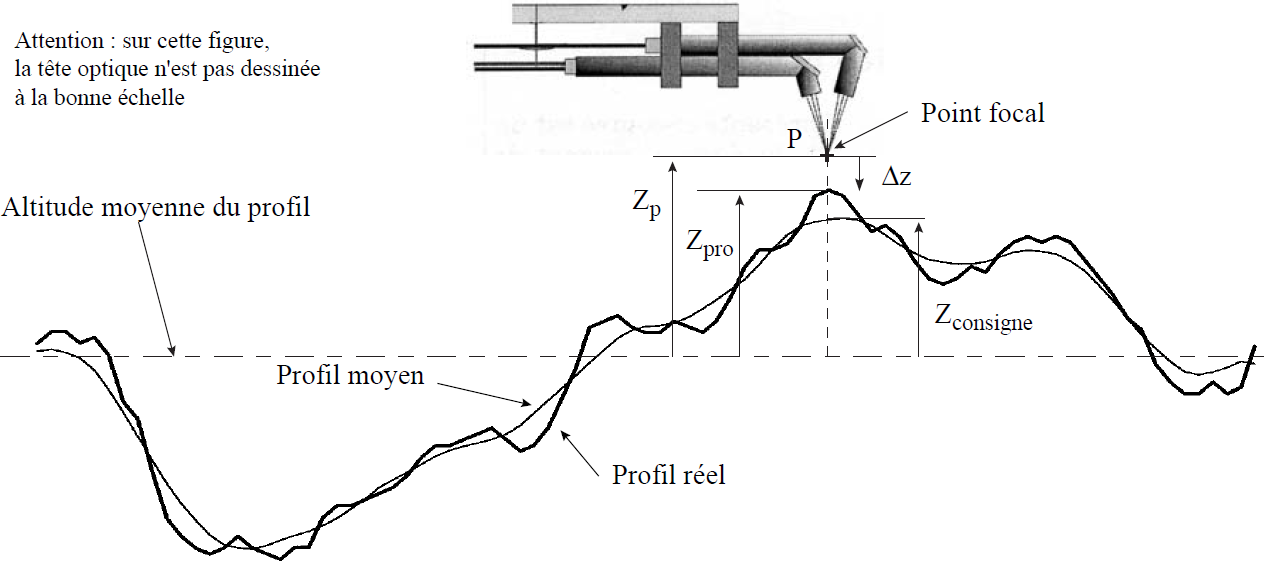
\includegraphics[width=.9\linewidth]{fig_08}
\captionof{figure}{F.A.S.T. \label{fig_08_quille}}
\end{center}

Parmi les moyens mis en œuvre, la chaîne de solides qui termine la chaîne d’énergie est représentée et modélisée sur le document « Annexe 1 ».

Cette chaîne est composée :
\begin{itemize}
\item du berceau $N$ encastré sur la coque du navire et dont le repère associé est RN : $\repere{O}{x_N}{y_N}{z_N}$;
\item de la quille 1 constituée du voile et du lest d’extrémité et dont le repère associé est R1 : $\repere{O}{x_1}{y_1}{z_N}$;
\item du vérin 2-4 constitué du piston 2 et du cylindre 4 et dont les repères associés sont respectivement R2 : $\repere{A_2}{x_2}{y_2}{z_2}$  et R4 : $\repere{C}{x_2}{y_2}{z_2}$  (la rotation relative 2-4 ne sera pas prise en compte dans l’étude et donc les bases de R2 et R4 seront confondues);
\item du vérin 3-5 constitué du piston 3 et du cylindre 5 et dont les repères associés sont respectivement R3 : $\repere{A_3}{x_3}{y_3}{z_3}$ et R5 : $\repere{B}{x_3}{y_3}{z_3}$  (la rotation relative 3-5 ne sera pas prise en compte dans l’étude et donc les bases de R3 et R5 seront confondues);
\item le paramétrage complet et la définition des liaisons entre ces solides figurent dans l’<< Annexe 1 >>.
\end{itemize}
%2-	
\section{Fonction FT1.2 : << Déplacer la quille>>. Fonction composante FT1.2.1 : << Alimenter : développer une puissance motrice suffisante >>}

L’objectif est de déterminer la puissance utile au déplacement de la quille et de la comparer à celle installée par le constructeur.

Dans cette partie, le modèle de calcul est celui fourni par l’ « Annexe 1 ». Le modèle utilisé est le modèle « plan », représenté Figure A2. 

Le bateau est à l’arrêt et son repère $R_N$ est galiléen. 

Lors de la commande de basculement de la quille, les vérins sont alimentés de telle sorte que : $F_{h2}>0$ et $F_{h3}=0$ (voir l’<< Annexe 1 >>). Le vérin 2-4 est alors moteur et le vérin 3-5 est libre.

Les liaisons sont parfaites. Le mouvement du fluide dans les diverses canalisations s’accompagne d’un phénomène de frottement visqueux  défini en << annexe 1 >>. L’eau exerce sur le voile de quille une action  hydrodynamique définie en << annexe 1 >>.

\subsection*{Validation de la puissance installée}
%Liminaire : 
%Question 5
\question{Exprimer les vitesses suivantes : $\vectv{G_1}{1}{N}$, $\vectv{G_2}{2}{N}$, $\vectv{G_3}{3}{N}$, $\vectv{A}{2}{4}$.}
%\vspace{-.4cm}
%\textit{\begin{itemize}
%\item en fonction de   et des paramètres géométriques utiles.
%b-   en fonction de ,  ,  et des paramètres géométriques utiles.
%c-   en fonction de ,  ,  et des paramètres géométriques utiles.
%d-   en fonction de .
%\end{itemize}}
%Soit E l’ensemble constitué des solides 1, 2, 3, 4 et 5.
%Expression des énergies cinétiques galiléennes (le repère RN est galiléen) des solides de E en mouvement.
%%Question 6
%Parmi celles développées par les solides de E, exprimer uniquement les suivantes: 
%
%a-	Energie cinétique galiléenne du solide 1 dans son mouvement par rapport à N, T(1/N), en fonction de  et des paramètres inertiels et géométriques utiles. 
%b-	Energie cinétique galiléenne du solide 2 dans son mouvement par rapport à N, T(2/N), en fonction de  ,  ,  et des paramètres inertiels et géométriques utiles. 
%c-	Energie cinétique galiléenne du solide 4 dans son mouvement par rapport à N, T(4/N), en fonction de  et des paramètres inertiels et géométriques utiles. 


%Evaluation des puissances développées par les actions mécaniques intérieures à E.
%%Question 7
%Recenser (notation P(i j/k)), puis exprimer les puissances non nulles développées par les actions mécaniques intérieures à E en fonction du (ou des) paramètre(s) propre(s)  à la liaison ou au mouvement concerné.
%
%Evaluation des puissances développées par les actions mécaniques extérieures à E.
%%Question 8
%Recenser (notation P(i j/N), puis exprimer les puissances galiléennes non nulles développées par les actions mécaniques extérieures à E. Chaque puissance sera exprimée à l’aide du (ou des) paramètre(s) propre(s)  à la liaison ou au mouvement concerné. Les notations utilisées sont celles des tableaux de l’ « Annexe 1 ».
%
%
%%Question 9
%Appliquer le théorème de l’énergie-puissance à E dans son mouvement par rapport à N. Ecrire ce théorème de façon globale en utilisant uniquement les notations précédentes, sans leur développement. Exprimer dans ces conditions la puissance motrice que fournit le vérin moteur en fonction du reste : équation (1).




On se place dans le cas où une commande en vitesse est générée à destination du vérin [2, 4]. Le vérin [3, 5]  est libre. Cette commande « en trapèze de vitesse» (voir figure A de l’ « Annexe 2 ») provoque le déplacement de la quille de la position $\theta_1 = 0\degres$ à la position $\theta_1= 45\degres$ en 4 secondes, le maintien de la quille dans cette position pendant 1 seconde puis le retour à la position $\theta_1 = 0$ en 4 secondes. Les phases d’accélération et de décélération (rampes) durent 1 seconde.

Un logiciel de calcul permet de tracer l’évolution temporelle des puissances mises en jeu. Ces puissances sont représentées sur le document « Annexe 2 ». 

%Question 10
\question{}
\vspace{-.4cm}
\textit{
\begin{enumerate}
\item Dans le but de chiffrer la valeur maximale de la puissance que doit fournir l’actionneur pour réaliser le mouvement prévu, tracer, à l’aide de l’« Annexe 2 », sur la figure R4 de la copie, l’allure de l’évolution temporelle de cette puissance. Pour cela, évaluer les valeurs aux instants $t = \SI{0}{s}$, $t = \SI{1}{s}$,     $t= \SI{3}{s}$ et $t = \SI{4}{s}$.
Sur cet intervalle $[0,\SI{4}{s}]$, évaluer, en kW, la valeur maximale de la puissance que doit fournir l’actionneur. Expliquer pourquoi le maximum de puissance est situé sur cet intervalle.
\item Le constructeur indique une puissance motrice installée sur son bateau de \SI{30}{kW}. 
Dans les hypothèses utilisées pour constituer le modèle de calcul, indiquer ce qui peut expliquer la différence  entre la valeur calculée et la valeur installée.
\end{enumerate}}

\begin{center}
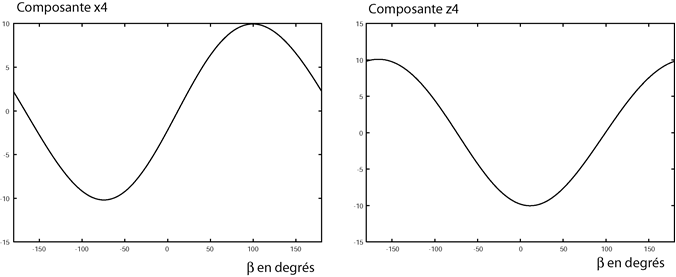
\includegraphics[width=.5\linewidth]{dr_04}
%\caption{Stabilité << de formes >> \label{fig_02_quille}}
\end{center}

\section{Fonction FT1.2.4 : « Transmettre l'énergie mécanique ». Fonction composante FT1.2.4.1 : « Guider la quille par rapport à la coque et maintenant le contact »}

L’objectif de cette partie est de valider la solution technologique de réalisation de la liaison pivot entre la quille et la coque. 
Le modèle de calcul pour cette partie est celui du document « Annexe 1 », version à 3 dimensions de la figure A1.% (voir aussi la copie).

Hypothèses :
\begin{itemize}
\item les liaisons sont toutes parfaites;
\item seul le vérin 2-4 est moteur ($F_{h3}=0$): l’action mécanique motrice est donnée par $\torseurstat{T}{\text{ph}}{2} = \torseurl{F_{h2}\vect{x_2}}{\vect{0}}{C}$;
\item les actions mécaniques de frottement visqueux provenant du déplacement du fluide dans les canalisations sont toutes négligées ($k=0$);
\item les actions hydrodynamiques sur le voile et le lest de quille sont également négligées;
\item les poids des éléments constitutifs des deux vérins sont négligés;
\item la variation de $\theta_2$ pour toute l’amplitude du mouvement de relevage de la quille est faible ; $\theta_2$ sera pris égal à 0 : les bases $B_2$,  $B_4$ et $B_N$ sont donc confondues. Cependant l’angle $\theta_1$ est différent de zéro.
\item les conditions de déplacement rendent négligeables les effets dynamiques. Les théorèmes de la statique seront donc utilisés dans la suite.
\end{itemize}
%Question 11
\question{En isolant le bon système, montrer que l’action de 2 sur 1 en A2 est représentable par le glisseur dont la forme sera notée : $\torseurl{F_{21}\vect{x_2}}{\vect{0}}{A_2}$ ou $\torseurl{F_{21}\vect{x_N}}{\vect{0}}{A_2}$ puisque $B_N = B_2$.}


%Question 12
\question{En isolant le bon système, exprimer, en fonction de $d$, $g$, $M_1$, et $F_{21}$, par ses éléments de réduction en $O$, dans la base $\base{x_N}{y_N}{z_N}$, le torseur d’action mécanique de N sur 1, $\torseurstat{T}{N}{1}_{\text{pivot}}$. }

La liaison pivot de N sur 1 est composée de deux paliers modélisés par une liaison sphère-cylindre et une liaison sphérique placées en parallèle (voir figure \ref{fig_09_quille}). La géométrie de l’assemblage est telle que : $\vect{OO_2}=e\vect{z_N}$; $\vect{OO_1}=-e\vect{z_N}$ avec $e=\SI{350}{mm}$.

\begin{figure}[!h]
\centering
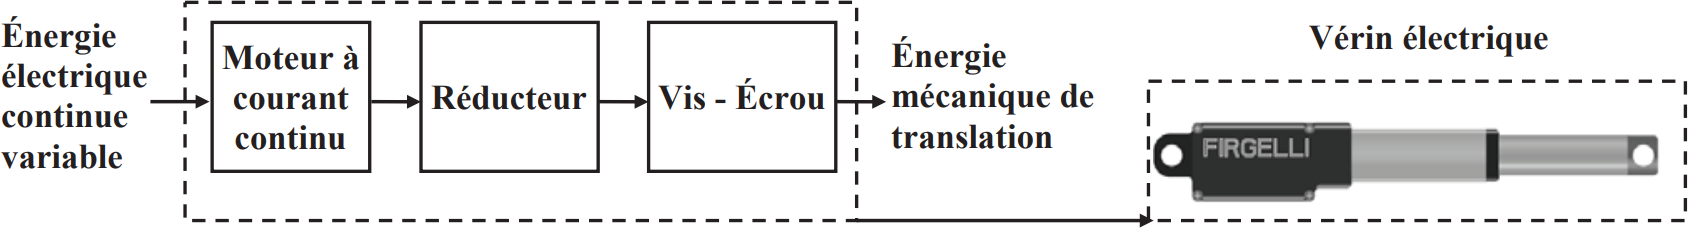
\includegraphics[width=.5\linewidth]{fig_09}
\caption{Composition de la liaison pivot 1/N. \label{fig_09_quille}}
\end{figure}


%Question 13
\question{Ecrire la relation liant les torseurs d’action mécanique $\torseurstat{T}{N}{1}_{\text{sphère-cylindre}}$, $\torseurstat{T}{N}{1}_{\text{sphérique}}$ et $\torseurstat{T}{N}{1}_{\text{pivot}}$. 
En déduire, par ses éléments de réduction en $O_1$, dans la base $B_N  \base{x_N}{y_N}{z_N}$, en fonction de $d$, $g$, $M_1$ et $F_{21}$, le torseur d’action mécanique de $N$ sur 1 en $O_1$, $\torseurstat{T}{N}{1}_{\text{sphère-cylindre}}$. }



On se place dans les conditions suivantes :
\begin{itemize}
\item la valeur maximale de l’action $F_{21}$ a été estimée dans l’étude précédente : $F_{21\text{Maxi}} = \SI{2e5}{N}$. De plus : $M_1 g = \SI{4,1e4}{N}$, $e = \SI{350}{mm}$ et $d = \SI{200}{mm}$.
\item les « paliers » sont constitués côté quille de contacts cylindriques de diamètre $d_c = \SI{80}{mm}$ et de longueur $L_c = \SI{50}{mm}$, $O_1$ étant dans le plan médian du cylindre de contact. Un coussinet de nylon sert d’interface entre la quille et le navire. Ce coussinet est caractérisé par sa pression de contact maximale admissible : $\indice{p}{adm} = \SI{50}{N/mm^2}$.
\end{itemize}

%Question 14
\question{Dans ces conditions, calculer la valeur de l’effort radial (perpendiculaire à l’axe géométrique du coussinet) qui sollicite ce coussinet en $O_1$.
Valider ensuite l’usage de ce coussinet de nylon à l’aide de l’ « Annexe 3 ».}



%%4
%\section{Fonction FT1.1.2 : « Traiter l'information ». Foction composante FT1.1.2.1 : « Gérer les cycles préprogrammés»}
%
%L’automate, qui réalise la fonction TRAITER l’information, a son activité décomposée en deux tâches selon le diagramme FAST de la Figure \ref{fig_10_quille}.
%
%
%
%La commande des manœuvres de la quille s’effectue via un pupitre (voir figure \ref{fig_11_quille}) placé à proximité du poste de barre à partir duquel le navigateur peut demander à l’automate de réaliser :
%•	Le déplacement de la quille d’un bord ou de l’autre selon une valeur de consigne.
%•	Des cycles préprogrammés comme celui de « virement de bord » et celui de « Relâcher ». Le cycle de virement de bord permet de placer la quille de façon symétrique à la position qu’elle occupait précédemment. Ce cycle est utilisé lorsque le navigateur change l’orientation du navire par rapport au vent lors d’un virement de bord. L’automate prend alors en charge intégralement la séquence de manœuvres de la quille, laissant le navigateur disponible pour les autres tâches.
%Le cycle « Relâcher » permet de déplacer la quille sous le seul effet de la pesanteur. La quille est ainsi manœuvrée sans utiliser l’énergie de la centrale hydraulique.
%L’automate est également interfacé via le réseau du navire à une base de données où sont stockés les paramètres des navigations précédentes (conditions météorologiques, performances du navire et angle de quille). Le navigateur peut ainsi intégrer les paramètres de la quille à l’ensemble des paramètres décisionnels qui lui permettent d’élaborer sa stratégie de navigation.
%L’automate gère également la centrale hydraulique qui met en pression l’huile utilisée dans les vérins de manœuvre de la quille.
%
%Deux capteurs renseignent l’automate :
%•	Un inclinomètre mesure l’angle de gîte du navire, information notée .
%•	Le capteur de position angulaire mesure l’angle d’inclinaison de la quille, grandeur notée mes().
%Le pupitre de commande est doté de quatre boutons poussoirs : 
%•	tr : Demande d’inclinaison sur tribord.
%•	b : Demande d’inclinaison sur bâbord.
%Un appui « bref » sur l’un ou l’autre de ces boutons provoque une évolution de l’angle de consigne de 1°, un appui « long » une évolution de 10°.
%•	vir : Demande du cycle « virement de bord ».
%•	rel : Demande du cycle « Relâcher ».
%Il comporte également un afficheur numérique permettant de visualiser soit l’angle d’inclinaison de la quille, soit la valeur de consigne lorsque le barreur agit sur « bâbord » ou « tribord » (variables b ou tr). 
%Le modèle de commande implanté dans l’automate est défini par les grafcets G1, G2, G3 et G4 de la copie.
%
%%Question 15
%A l’instant t0, la situation du graphe de commande est {0, 30} et la quille est alors inclinée de +20°. Le navigateur donne une série d’impulsions sur b et tr conformément au chronogramme donné sur le document réponse R5 de la copie. 
%En analysant le modèle de commande, compléter le graphe des évolutions temporelles de la consigne angulaire c donné sur le document réponse R5 jusqu’à l’instant t3 et donner la valeur obtenue pour c, et ce, sans se préoccuper de la façon dont la partie opérative réagit à cette consigne.
%
%
%
%%Question 16
%La situation de départ est {0, 30} et la quille est alors inclinée de +40°. Le navigateur donne la consigne de virement de bord, vir.
%\question{Donner la liste des situations présentées par le modèle de commande jusqu’au retour dans la situation identique à celle de départ.}
%\question{En considérant que la chaîne de commande de la quille est précise, donner la valeur angulaire que représente mes() en fin de ce cycle.}


%5-	
\section{Fonction FT1.1.2 : « Traiter l'information ». Fonction composante FT1.1.2.2 : « Respecter la consigne angulaire de position ». Validation du cahier des charges}

Afin de garantir sa répétabilité, la mise en position angulaire de la quille fait l’objet d’un contrôle par une boucle d’asservissement, dont le cahier des charges est donné ci-dessous.

\subsection*{Cahier des charges}

\begin{center}
\begin{tabular}{lll}
\cline{2-3}
& Critères & Niveau \\
\hline
Stabilité	 & 	C11 Marge de gain 		& $\SI{10}{dB}$ \\
	 &	C12 Dépassement vis-à-vis d’une entrée en échelon 	& Aucun \\
\hline 		
Rapidité &	C21 Temps de réponse à 5\% 	& \SI{4}{s} maxi	\\
	&	C22 Vitesse angulaire de rotation de la quille	& $\SI{8}{\degres/s}$ maxi \\
\hline
Précision &	C3 Erreur statique vis-à-vis d’une entrée en échelon	& nulle \\
\hline
\end{tabular}
\end{center}

La quille est manœuvrée par deux vérins hydrauliques. Chacun d’eux est piloté par une servovalve de débit. Ce composant délivre un débit $q(t)$ proportionnel à sa tension de commande $v(t)$. Lors d’une manœuvre de quille un seul de ces vérins est moteur et alimenté en pression via sa servovalve. L’autre est laissé dans une configuration où sa tige est libre de tout mouvement. Le déplacement terminé, la quille est verrouillée en position par un système de blocage non étudié dans ce sujet qui interdit toute circulation de fluide entre vérins et servovalves. L’angle de rotation de la quille par rapport au bâti est mesuré par un capteur potentiométrique.

%5.1 
\subsection{Modélisation du vérin}
Lors d’un déplacement de la quille, les mouvements d’oscillation du cylindre de vérin par rapport à la coque étant de faible amplitude et s’effectuant à de faibles vitesses, on se place dans une situation où le corps de vérin est considéré comme fixe. La tige est alors considérée en mouvement de translation galiléen.
On considère également que les mouvements étudiés sont de petits mouvements autour d’une position moyenne et que l’hypothèse des conditions initiales nulles est valide. Dans ces conditions, le comportement du vérin est défini par le modèle continu ci-dessous  figure \ref{fig_12_quille}.

\begin{figure}
\centering
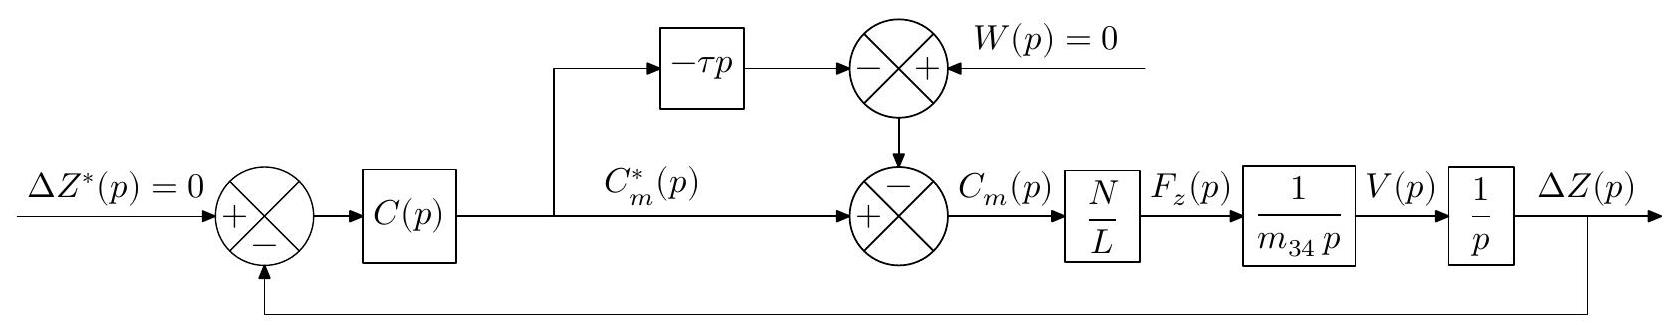
\includegraphics[width=.8\linewidth]{fig_12}
\caption{Schéma-blocs du vérin \label{fig_12_quille}}
\end{figure}


$q(t) = S\dfrac{\d x(t)}{\d t}+\dfrac{V}{2B}\dfrac{\d \sigma(t)}{\d t}$ et
$ M \dfrac{\d^2 x(t)}{\d t^2} = S\sigma(t) - kx(t) - \lambda\dfrac{\d x(t)}{\d t}-f_R (t)$.   


\begin{center}
\begin{tabular}{cp{12cm}{c}}
\hline
1 & Définition & 2 \\
\hline 
$q(t)$ 		& Débit d’alimentation du vérin ($\si{m^3.s^{-1}}$)			& $Q(p)$ \\
$\sigma(t)$	& Différence de pression entre les deux chambres du vérin ($\si{Pa}$)	& $\Sigma(p)$\\
$x(t)$		& Position de la tige du vérin ($\si{m}$)					& $X(p)$ \\
$f_R(t)$		& Composante selon l’axe de la tige de vérin de la 
			résultante du torseur d’inter-effort de la liaison pivot 
			entre tige et quille. ($\si{N}$)					& $F_R(p)$ \\
\hline
\end{tabular}

1 : Variable temporelle et 2 : Transformée de Laplace correspondante.
\end{center}

\begin{center}
Constantes : Définitions et unités (toutes les constantes sont positives)
\begin{tabular}{cp{12cm}}
\hline
S & 	Section du vérin ($\si{m^2}$) \\
k & 	Raideur mécanique du vérin ($\si{N.m^{-1}}$) \\
V & 	Volume d’huile de référence ($\si{m^3}$) \\		
B &	Coefficient de compressibilité de l’huile ($\si{N.m^{-2}}$)\\
M &	Masse équivalente à l’ensemble des éléments mobiles ramenée sur la tige de vérin ($\si{kg}$) \\
$\lambda$  & Coefficient de frottements visqueux ($\si{N.m^{-1}.s}$) \\
\hline
\end{tabular}
\end{center}



%Question 17
\question{Donner les expressions des fonctions de transfert $A1$, $A2$, $A3$ et $A4$ en fonction de la variable complexe p et des constantes.}

%Question 18
Le schéma-bloc de la figure \ref{fig_12_quille} peut se mettre sous la forme de la figure \ref{fig_13_quille}.

\question{Donner les expressions des fonctions de transfert $H_1$ et $H_2$ en fonction de $A1$, $A2$, $A3$ et $A4$, puis de la variable $p$ et des constantes.}


\begin{figure}[!h]
\centering
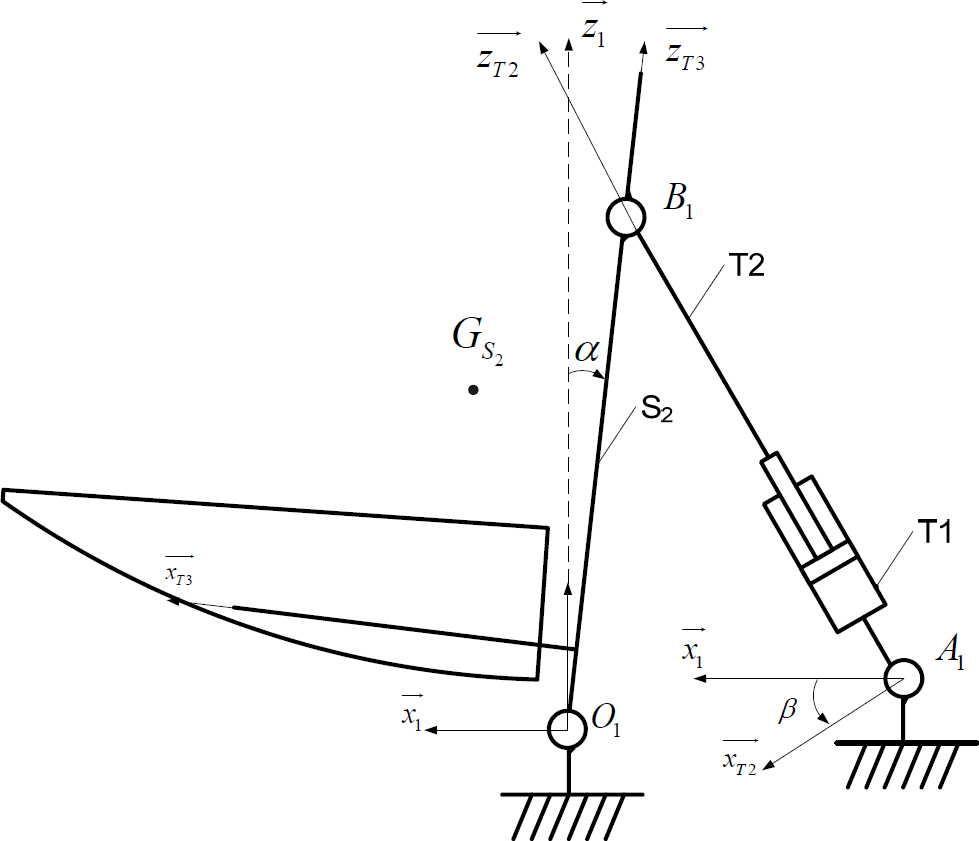
\includegraphics[width=.5\linewidth]{fig_13}
\caption{Schéma-blocs réduit du vérin. \label{fig_13_quille}}
\end{figure}


%Question 19
\question{Pour ce vérin non perturbé ($F_R=0$), donner sa fonction de transfert $\dfrac{X(p)}{Q(p)}$ en fonction de la variable $p$ et des constantes.}

Le schéma d’asservissement de la position angulaire de la quille représenté figure \ref{fig_14_quille} ci-dessous sera utilisé pour la suite des questions. La perturbation représentée par $F_R(p)$ ne sera pas prise en compte.

\begin{figure}[!h]
\centering
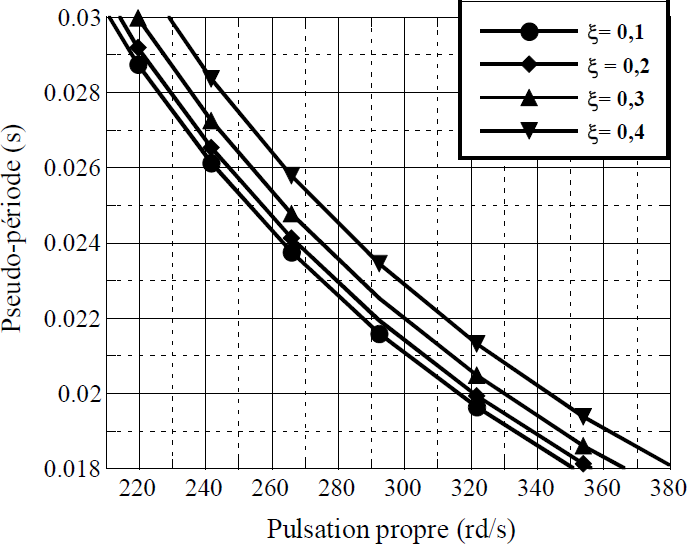
\includegraphics[width=\linewidth]{fig_14}
\caption{Schéma-blocs de la commande complète. \label{fig_14_quille}}
\end{figure}


\begin{center}
\begin{tabular}{lll}
\hline
Variable temporelle	& Définition (unité)				& Transformée de Laplace \\
\hline
$\theta_c(t)$		& Consigne de position angulaire (\degres)	& $\Theta_c(p)$ \\
$\theta(t)$		& Position angulaire de la quille (\degres)	& $\Theta(p)$ \\
$v(t)$			& Tension de commande de la servovalve ($V$)	& $V(p)$ 	\\
$v_c(t)$		& Tension image de la consigne ($V$)		& $V_c(p)$ 	\\
$v_m(t)$ 	 	& Tension image de la position ($V$)		& $V_m(p)$ 	\\
\hline
\end{tabular}
\end{center}



\begin{center}
Fonctions de transfert : définitions (unité)
\begin{tabular}{lp{14cm}}
\hline
$K_c$			& Gain du capteur angulaire potentiométrique ($\si{V/\degres}$) \\
$K_c'$			& Gain du bloc d’adaptation réglé tel que $K_c' = K_c = \SI{1,1}{V/\degres}$ \\
$C(p)$			& Correcteur de position 	\\
$\indice{H}{CIN}$ 	& Fonction de transfert de la chaine de transformation de mouvement 
			dont la loi d’entrée/sortie est supposée linéaire dans le domaine d’utilisation.                
			 $\indice{H}{CIN} = K_{\theta}$ ($\si{\degres.m^{-1}}$) \\
$\indice{H}{sv}$	& Fonction de transfert de la servovalve  \\
\hline
\end{tabular}
\end{center}




%5.2 
\subsection{Modélisation de la servovalve : comportement pour une commande de grande amplitude}

La servovalve présente un fonctionnement non-linéaire provenant d’un phénomène de saturation qui est défini par la courbe de la figure \ref{fig_15_quille} donnant les évolutions du débit $q(t)$ fourni par la servovalve en fonction de sa tension de commande $v(t)$. 

\begin{figure}[H]
\centering
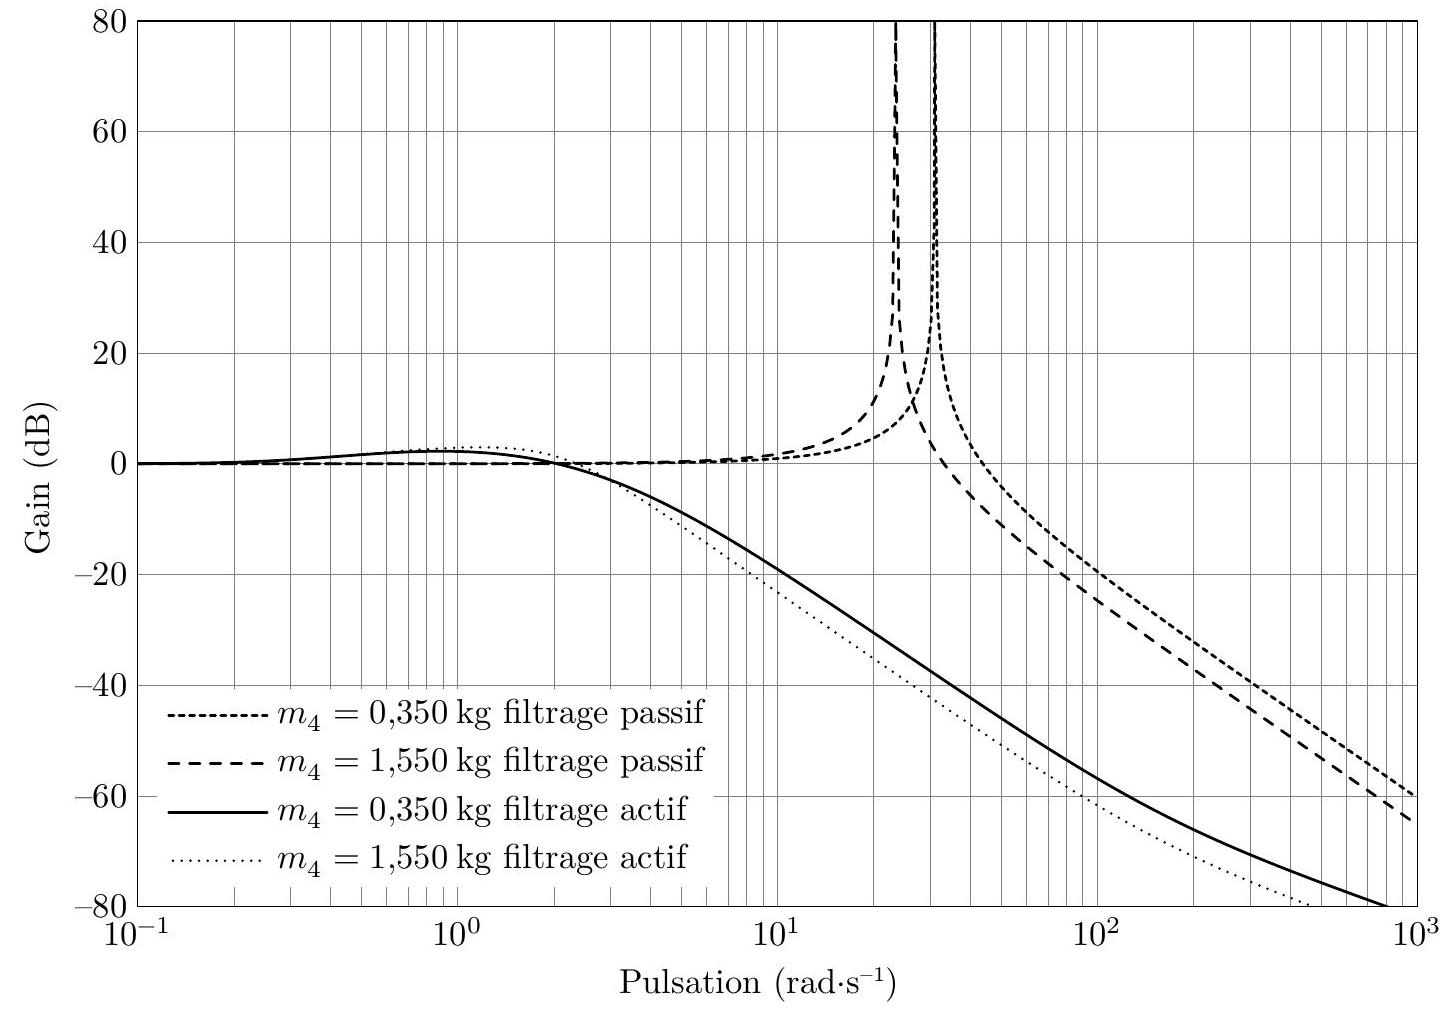
\includegraphics[width=.5\linewidth]{fig_15}
\caption{Fonctionnement de la servovalve. \label{fig_15_quille}}
\end{figure}

Ainsi :
\begin{itemize}
\item pour $v(t) > -\indice{v}{max}$ et $v(t) < \indice{v}{max}$ : 
$\indice{H}{sv} = \indice{K}{sv}$  ($\si{m^3.s^{-1}.V^{-1}}$);
\item pour $v(t) < -\indice{v}{max}$: $q(t) = -\indice{q}{max}$
\item pour $v(t) > \indice{v}{max}$ : $q(t) = +\indice{q}{max}$, $\indice{v}{max} = \SI{10}{V}$.
\end{itemize}

Le système n’est pas encore corrigé, $C(p) =1$ et on souhaite simuler le fonctionnement où le navigateur 
veut déplacer la quille avec une consigne angulaire de position de $45\degres$. Cette demande est modélisée 
par une consigne  $\theta_c(t)$ en échelon, soit : $\theta_c(t)=\theta_0 u(t)$
avec $\theta_0= 45\degres$ 
et $u(t) = 0$ pour $t < 0$ et $u(t) = 1$ pour $t > 0$. La figure R6 du document réponse présente dans 
ces conditions les évolutions temporelles de deux grandeurs de la boucle d’asservissement, le débit 
sortant de la servovalve $q(t)$ et la position angulaire de la quille $\theta(t)$.


%Question 20
Sur cette figure R6, la courbe représentative de $q(t)$ présente un palier où $q(t)$ garde une valeur constante.    
\begin{center}
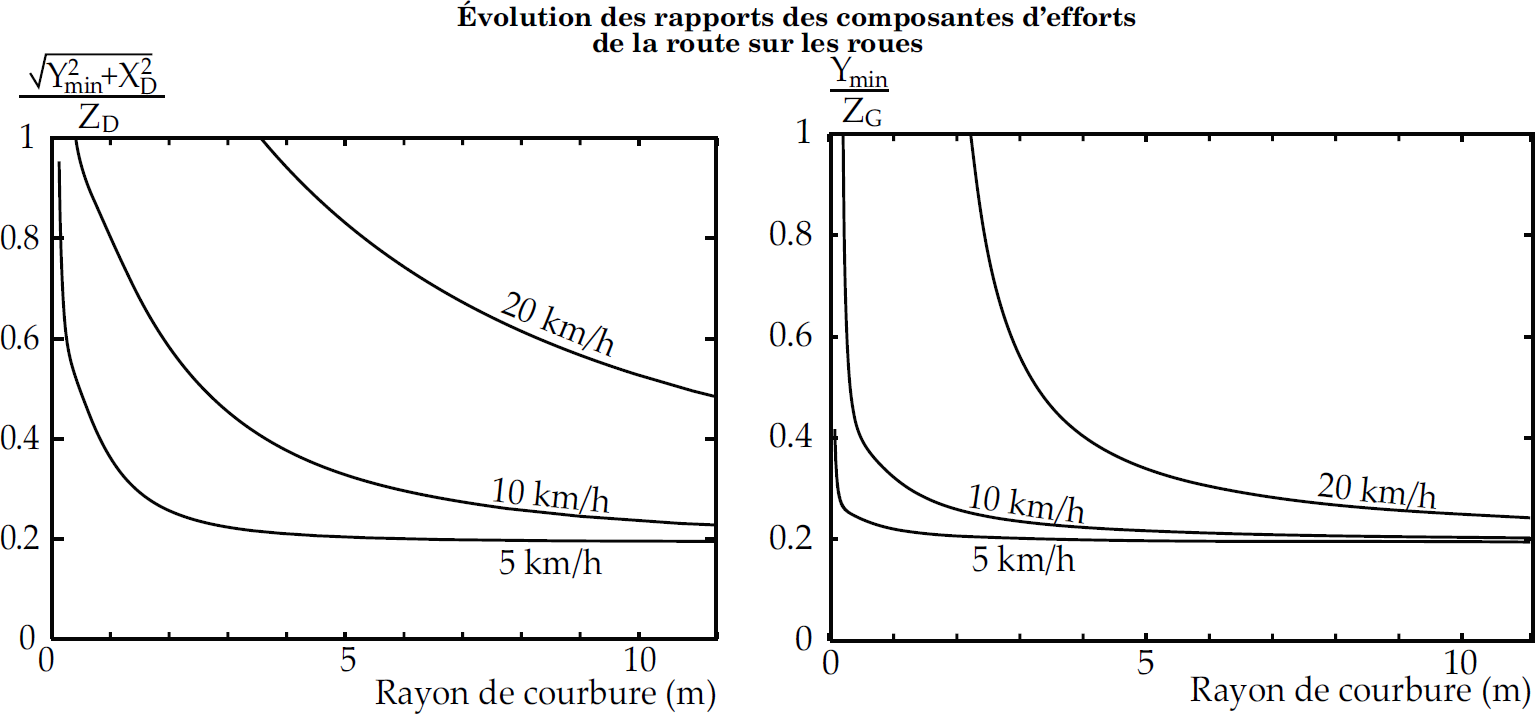
\includegraphics[width=.6\linewidth]{dr_06}
%\caption{Stabilité << de formes >> \label{fig_02_quille}}
\end{center}

\question{A l’aide de la caractéristique de la servovalve :}
\vspace{-.4cm}
\textit{
\begin{itemize}
\item Justifier ce palier et donner la valeur numérique de $\indice{K}{SV}$.
\item Indiquer sur la figure R6 l’intervalle de temps où le retour d’information a une influence sur la commande du vérin et celui où il n’en a pas. Associer à chacun de ces intervalles le modèle utile : modèle en « boucle fermée » ou en « boucle ouverte ».
\end{itemize}}

\vspace{.5cm}

%Question 21
\question{Montrer, en précisant le ou les critères mis en défaut, que le cahier des charges n’est pas respecté au niveau des critères « vérifiables ». }


\subsection{Comportement pour une commande de faible amplitude}
On étudie la réponse du système non corrigé ($C(p) = 1$) à une entrée échelon de 5\degres d’amplitude avec $F_R = 0$. Le modèle de travail qui a permis de tracer les courbes de la figure R6 est :

$$ 
\indice{H}{BO}(p)=\indice{K}{SV}H_1 H_2 K_{\theta} K_c 
\quad \quad 
\indice{H}{BO}(p)=\dfrac{2,2}{p\left( 1+0,12p+0,04 p^2\right)}.
$$

%Question 22
\question{}
\vspace{-.4cm}
\textit{
\begin{enumerate}
\item Pour l’entrée définie ci-dessus, déterminer la valeur de la tension $v(t)$ à l’instant initial $t=0^{+}$, $v(0^{+})$.
\item Montrer que tout au long de ce fonctionnement, la servovalve fonctionnera sans saturer.
\item De quelle hypothèse générale d’étude des systèmes asservis ce constat participe-t-il ?
\end{enumerate}}



Une simulation de la réponse indicielle à cet échelon de 5\degres d’amplitude a permis de tracer les courbes de la figure \ref{fig_16_quille}, obtenues pour deux valeurs du correcteur proportionnel :
\begin{itemize}
\item $C(p) = 1$ : la courbe présente des dépassements, le critère C12 n’est pas validé.
\item $C(p) = 0,44$ : tous les critères du domaine temporel sont vérifiés (C12, C21, C22, C3).
\end{itemize}

À l’utilisation, le correcteur proportionnel réglé à 0,44 n’a pas donné satisfaction car le mouvement saccadé de la quille dû aux fluctuations de sa vitesse de rotation générait dans certaines conditions de navigation des perturbations compromettant la stabilité de route du navire. L’examen attentif de cette réponse indicielle fait apparaître la persistance d’un phénomène oscillatoire dont l’origine supposée se trouve dans le caractère résonant du vérin.

%Question 23
\question{}
\textit{
\begin{itemize}
\item Tracer sur les figures R7 et R7 ’de la copie, les diagrammes d’amplitude asymptotiques de Bode de 
$\indice{H}{BO}(p)$ en indiquant les valeurs numériques associées aux points particuliers et la valeur des pentes.
\item Déterminer par calcul la pulsation de résonance $\omega_r$ de cette fonction de transfert.
\item Evaluer littéralement puis numériquement à cette pulsation $\omega_r$ la différence, notée $\Delta K$ et exprimée en dB, entre l’amplitude de résonance et l’amplitude évaluée par le diagramme asymptotique.
\end{itemize}}

\begin{figure}[!h]
\centering
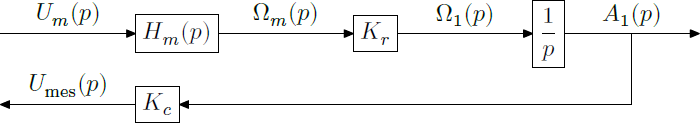
\includegraphics[width=.7\linewidth]{fig_16}
\caption{Réponse indicielle à un échelon de 5\degres. \label{fig_16_quille}}
\end{figure}

Pour éliminer le phénomène de résonance, on recherche l’expression de $C(p)$ permettant d’abaisser l’amplitude de $\Delta K$ à la pulsation $\omega_r$. Le concepteur a choisi un correcteur à retard de phase de fonction de transfert $C(p)=\indice{K}{COR}\dfrac{1+Tp}{1+bTp}$ avec $b>1$. Ce correcteur présente un extremum de la courbe de phase à la pulsation $\omega^*$ tel que : $\sin\left( \phi\left(\omega *\right)\right)=\dfrac{1-b}{1+b}$ et $\omega^*=\dfrac{1}{T\sqrt{b}}$.     
L’étude consiste à déterminer les valeurs de $T$ et $b$.

%Question 24
\question{}
\textit{
\begin{enumerate}
\item Tracer sur la figure R8 de la copie, les diagrammes d’amplitude et de phase (asymptotiques et allure de la courbe réelle) de Bode de ce correcteur pour $\indice{K}{COR} =1$. Préciser les expressions littérales des pulsations caractéristiques.
\item 
Déterminer alors en fonction de $b$, l’amplitude $\left| C(j\omega^*)\right|_{dB}$ à la pulsation notée $\omega^*$.
\end{enumerate}}


%Question 25
\question{Pour $\indice{K}{COR} =1$, en faisant correspondre la pulsation de résonance $\omega_r$ de $\indice{H}{BO}$ à $\omega^*$ , calculer b pour que « l’excès » de gain $\Delta K$ soit compensé par le correcteur et calculer la valeur de $T$. Calculer ensuite le supplément de déphasage introduit par le correcteur à la pulsation $\omega^*$.}

La réponse indicielle correspondant à ce réglage (entrée échelon de 5\degres d’amplitude) est donnée sur le document réponse figure R9. Le gain $\indice{K}{COR}$ a été déterminé de façon à satisfaire les critères C11 et C12.

%%Question 26 
\question{Déterminer la vitesse de rotation angulaire maximale de la quille obtenue avec ce réglage du correcteur.}

\question{Validez les critères C21 et C22 en laissant vos constructions apparentes.}
